\chapter{CONTROL UNDER PARTIAL OBSERVABILITY}
\label{ch:pomdp-control}

\aigen{\emph{This chapter is based on joint work with Ziping Xu \citep{tan2026pomdp}: Kevin Tan and Ziping Xu, ``From POMDP Theory to Deep RL with Particle Filters,'' in Advances in Neural Information Processing Systems 39 (NeurIPS), 2026.}}

\todoresolve{CHAPTER 8 COMPLETES THE PARTIAL-OBSERVABILITY PROGRESSION WITH CONTROL AND PLANNING (TAN AND XU, NEURIPS 2026).}


\section{Introduction}


Partially observable Markov decision processes (POMDPs) provide a standard framework for sequential decision making under latent state uncertainty \citep{kaelbling1998planning}. They are a natural model for problems in robotics, healthcare, recommendation, and other settings \citep{hauskrecht2000planning,pineau2003point} where the learner must act using only indirect and noisy observations of the underlying system. 
In principle, optimal control in a POMDP can be reduced to planning in the belief-state MDP, where the belief is the posterior distribution over latent states given the observation history \citep{cassandra1994acting,kaelbling1998planning}. This makes model-based RL especially natural in POMDPs: to act under a belief, the learner must already learn a model rich enough to perform filtering, and this same model can be used for planning. 

However, the belief state reduction does not remove the main computational and learning difficulties. An online model-based decision maker must simultaneously (i) learn the unknown model, (ii) maintain a posterior over latent states online, and (iii) plan over this continuous belief space. These three tasks---\textit{learning, inference, and planning}---interact in a way that makes exact online control in POMDPs intractable in both computation and sample complexity in general \citep{papadimitriou1987complexity} without special structure, motivating a large literature on \textit{approximate} methods for each component individually. 

Existing methods typically make one component of the above POMDP pipeline tractable while leaving the others either computationally expensive or theoretically uncontrolled. For instance, on the planning side, Monte Carlo tree search has led to scalable online POMDP solvers such as Partially Observable Monte Carlo Planning (POMCP), sparse tree search, and progressive widening methods \citep{silver2010monte,lim2021sparse,sunberg2018online}. However, these are primarily planning algorithms under a known generative model, and do not natively provide end-to-end learning guarantees for unknown latent dynamics.
A more aggressive approximation is QMDP, which replaces the belief-MDP continuation value by the fully observed MDP value averaged under the current belief \citep{littman1995learning}. QMDP is computationally efficient but can introduce substantial bias. Existing theory gives limited guidance on when this bias is small or how it can be mitigated. 
Regarding inference, particle filters, a.k.a. sequential Monte Carlo (SMC), provide a flexible approximation to Bayesian filtering in nonlinear non-Gaussian systems \citep{crisan2002survey,whiteley2013stability}, but SMC theory for POMDPs \citep{lim2021sparse,lim2023optimalityparticlepomdp} has not been fully integrated with approximate online planning and model learning. On learning, recent theoretical work has made significant progress on sample-efficient model estimation for POMDPs. \cite{liu2022partially,liu2023optimistic} develop Optimistic MLE as a generic model-based algorithm with polynomial sample complexity for a broad class of POMDPs. These results establish statistical feasibility under exact or abstract planning oracles. They do not specify how to perform approximate filtering or planning with the learned model in a computationally practical way.

A separate practical line of work uses recurrent policies or differentiable planning modules. Recurrent model-free deep RL methods, such as GRU or LSTM-based PPO and Q-learning variants, can perform well empirically under partial observability, but their hidden states are difficult to interpret as beliefs and are hard to analyze theoretically. QMDP-net takes a more structured approach by embedding approximate Bayesian filtering and QMDP planning into a differentiable architecture \citep{karkus2017qmdpnet}. This is closer in spirit to our goal: combine model learning, belief state inference, and planning in a way that resembles modern deep learning practice, while maintaining provable guarantees. However, the approximation error of learned variational or differentiable filtering is difficult to control. Our view is that using SMC as the filtering primitive yields a more principled bridge: it is compatible with learned latent dynamics and has well-developed stability and approximation theory \citep{crisan2002survey,whiteley2013stability}. 

In summary, existing work advances individual components---planning, inference, or learning---but no current method provides a unified pipeline that combines all three with both computational practicality and end-to-end theoretical guarantees. This leaves open the central question
\begin{center}
    \textit{Can we design a practical model-based deep RL pipeline for POMDPs
that still admits end-to-end theoretical guarantees?}
\end{center}


\subsection{Our Contributions}

This chapter develops a practical and analyzable route from POMDP theory to model-based deep RL. We answer the central question by developing a model-based learning-inference-planning pipeline for POMDPs (\aigen{Algorithm~\ref{alg:pf_mcts}}) that is compatible with deep RL practice. Our contributions are:
\begin{enumerate}
    \item \textbf{A practical inference-learning-planning pipeline.} We propose an online algorithm that learns a latent dynamics model, tracks the current belief with particles, and plans under this belief. Each is modular and can be instantiated with standard deep RL primitives.


    \item \textbf{A controlled alternative to full belief-tree planning.} Instead of treating the particle belief as the planning state, we plan particle-wise and average action-values of the fully observable MDP. This gives a practical middle ground between expensive belief-tree search and cheap but potentially biased QMDP. Our analysis shows that the bias decays geometrically after $d$ steps of belief-MDP lookahead. For cheaper state-level planners, we show that QMDP is exact for the belief-linear component of the value and fails only through an uncertainty-sensitive residual, clarifying when the approximation is small.

    \item \textbf{An end-to-end regret guarantee.}
    We prove a regret bound that decomposes performance loss into model estimation error, particle filtering error, Monte Carlo rollout error, and QMDP structural bias. The bound makes explicit how sample size, particle budget, rollout budget, and planning depth jointly control performance.

    \item \textbf{A bridge to deep RL practice.}
    Compared with theoretical POMDP learning algorithms that rely on exact POMDP solvers or posterior sampling over parameters, our approach uses MPC-style online planning, approximate filtering, and critic bootstrapping. These are standard primitives in model-based deep RL, while remaining explicit enough to support theoretical analysis. We instantiate our algorithm in an MPC-based deep RL implementation and evaluate it on a variety of POMDP environments, demonstrating its practicality. 
\end{enumerate}



Overall, this chapter argues that particle filtering can serve as a practical bridge between POMDP theory and deep RL. It gives a belief representation that is explicit enough to analyze, flexible enough for nonlinear latent dynamics, and compatible with MPC-style planning and learned critics. This yields a route to online POMDP learning that is closer to modern model-based RL than exact belief-space planning, while providing a transparent theoretical account that lets users trace each source of approximation error and make informed design choices.


The rest of this chapter is organized as follows. Section~\ref{sec:problem} introduces the online learning problem and the regret criterion in the belief-state MDP. Section~\ref{sec:algorithm} presents \aigen{Algorithm~\ref{alg:pf_mcts}}, describing the finite-depth belief-tree planning subroutine (\aigen{Algorithm~\ref{alg:mctq}}) and the full online pipeline. Section~\ref{sec:analysis} develops the error analysis: we decompose the regret into four traceable terms, analyze the structural QMDP bias and its variance interpretation, bound each error source, and combine them into the end-to-end regret guarantee. We conclude with case studies on LQG, contextual MDPs, and smooth-value POMDPs that illustrate when the QMDP approximation is benign.


\section{Problem Formulation}
\label{sec:problem}


\begin{figure}[t]
    \centering
    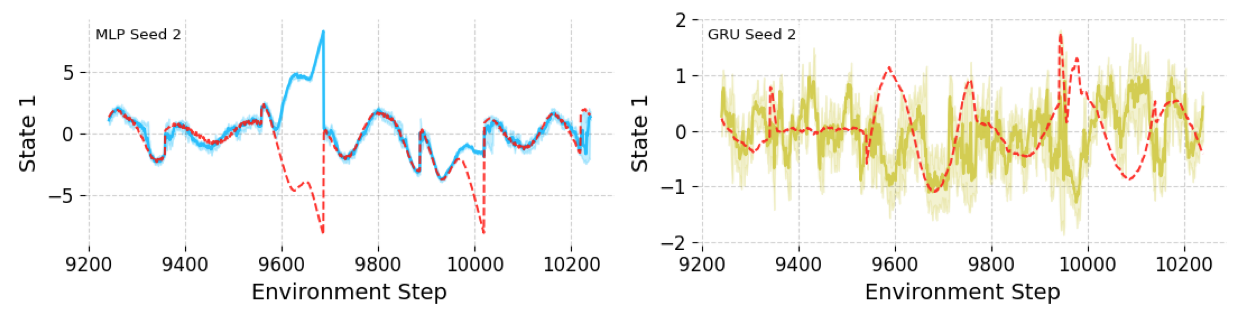
\includegraphics[width=\linewidth]{figures/ch08/Figures/lqr_posterior_small.png}
    \vspace{-4ex}
    \caption[Particle beliefs for the unobserved velocity of a double-integrator LQR]{Particle beliefs for the unobserved velocity of a double integrator LQR over the last 1000 steps. Mean, 10th and 90th quantiles visualized. Beliefs track the state when the system is stable.}
    \label{fig:lqr-posterior-small}
\end{figure}


We study online reinforcement learning in a partially observable environment with unknown dynamics. Since the latent state is hidden, the natural state variable for control is the belief, the posterior distribution of the latent state given the history. We begin by introducing the POMDP model and the associated belief-state dynamics.
Figure~\ref{fig:lqr-posterior-small} shows a particle approximation of such a belief for a partially observed double integrator (Section~\ref{ch08:sec:experiments}).

% \textbf{Notation.} For a measurable space $\mathcal X$, let $\Delta(\mathcal X)$ denote the set of probability distributions over $\mathcal{X}$.

\paragraph{Parameterized POMDP model.}
For each parameter $\theta \in \Theta$, let $\mathcal M_{\theta} = (\gS,\gA,\gO, P_{\theta}, Z_{\theta}, r,\gamma,b_0)$ be an infinite-horizon discounted POMDP, where $\gS$ is the latent state space, $\gA$ is the action space, and $\gO$ is the observation space. The controlled state transition kernel is $P_{\theta}(\cdot \mid s,a) \in \Delta(\gS)$, the observation kernel is $Z_{\theta}(\cdot \mid s') \in \Delta(\gO)$, the reward function is $r:\gS\times\gA\to [0, R_{\max}]$, the discount factor is $\gamma\in(0,1)$, and $b_0\in\Delta(\gS)$ is the initial belief. The true environment is specified by an unknown true parameter $\theta^\star$, and we write $\gM^{\star} := \gM_{\theta^\star}$. Here, for a measurable space $\mathcal X$, $\Delta(\mathcal X)$ denotes the set of probability measures on $\mathcal{X}$, and beliefs $b\in\Delta(\gS)$ are written as measures $b(\mathrm ds)$ throughout.

\paragraph{Generative process and belief states.}
At each time $t=0,1,2,\ldots$, the latent state, observation, and reward evolve according to
\begin{equation}\label{eq:generative}
S_{t+1}\sim P_{\theta^\star}(\cdot \mid S_t,A_t),\qquad
O_{t+1}\sim Z_{\theta^\star}(\cdot \mid S_{t+1}),\qquad
R_t = r(S_t,A_t).
\end{equation}
The learner does not observe $S_t$. Instead, decisions are based on the entire history up to time $t$ denoted by $H_t := (O_{1:t},A_{0:t-1},R_{0:t-1})$. Here $O_t$ is available before choosing $A_t$. A possibly randomized policy is a sequence $\pi=\{\pi_t\}_{t\ge0}$ such that $\pi_t(\cdot \mid H_t)\in\Delta(\gA)$.

\textbf{Belief states and Bayes filtering.} Fix a candidate parameter $\theta$. The corresponding belief state at time $t$ is the posterior distribution $b_t^\theta(\cdot) := \mathbb P_{\theta}(S_t\in\cdot \mid H_t)$. When $\theta=\theta^\star$, we write $b_t := b_t^{\theta^\star}$ for the true belief. Given a belief $b\in\Delta(\gS)$ and action $a\in\gA$, define the one-step predictive state distribution and the corresponding predictive observation law respectively by
\begin{equation}\label{eq:predictive_belief}
\tilde b_{\theta}(\cdot \mid b,a)
:= \int_{\gS} P_{\theta}(\cdot \mid s,a)\, b(\mathrm ds),  \qquad p_{\theta}(\cdot \mid b,a)
:= \int_{\gS} Z_{\theta}(\cdot \mid s')\, \tilde b_{\theta}(\mathrm ds' \mid b,a).
\end{equation}
After observing $o\in\gO$, the posterior is updated through the Bayes filter (which we later approximate)
\begin{equation}\label{eq:bayes_update}
\tau_{\theta}(b,a,o)(\mathrm ds) := \frac{Z_{\theta}(o \mid s)\, \tilde b_{\theta}(\mathrm ds \mid b,a)} {\int_{\gS} Z_{\theta}(o \mid s')\, \tilde b_{\theta}(\mathrm ds' \mid b,a)}.
\end{equation}

\paragraph{Belief-MDP value functions.}
The reward associated with belief $b$ and action $a$ is $r(b,a) := \E_{s \sim b}[r(s,a)]$. We assume throughout that $\gA$ is finite and that $|r(s,a)|\le R_{\max}$ for all $(s,a)\in\gS\times\gA$.

For each $\theta$, the POMDP induces a fully observed MDP on $\Delta(\gS)$. For any bounded measurable function $V:\Delta(\gS)\to\mathbb R$, define the belief-MDP Bellman operator
\begin{equation}\label{eq:bellman_operator}
(\gT_{\theta}V)(b)
:=
\max_{a\in\gA}
\left\{
r(b,a)+\gamma \int_{\gO} V\big(\tau_{\theta}(b,a,o)\big)\, p_{\theta}(o \mid b,a)\, \mathrm do
\right\}.
\end{equation}
Let $V_{\theta}^{\star,B}$ denote the unique fixed point of $\gT_{\theta}$. The optimal belief-state action-value function is
\begin{equation}\label{eq:Qstar_belief}
Q_{\theta}^{\star,B}(b,a)
:=
r(b,a)+\gamma \int_{\gO} V_{\theta}^{\star,B}\big(\tau_{\theta}(b,a,o)\big)\, p_{\theta}(o \mid b,a)\, \mathrm do,
\text{ and }
V_{\theta}^{\star,B}(b)=\max_{a\in\gA}Q_{\theta}^{\star,B}(b,a).
\end{equation}
More generally, for a policy $\pi$ acting on histories, let $V_{\theta}^{\pi,B}(b)$ denote the corresponding discounted value in the belief-MDP when the initial belief is $b$. Furthermore, we let $Q^{\star, S}_{\theta}$ and $V^{\star, S}_{\theta}$ denote the value function of the fully observable MDP.

% \paragraph{Fully observable MDP under parameter $\theta$.}
% In addition to the belief-MDP, each parameter $\theta$ also defines a fully observable discounted MDP on the latent state space $\gS$ with transition kernel $P_{\theta}$ and reward $r$. This MDP will serve as a planning surrogate later in the paper. For any bounded measurable $v:\gS\to\mathbb R$, define
% \begin{equation}\label{eq:fully_observable_bellman}
% (\gT_{\theta}^S v)(s)
% :=
% \max_{a\in\gA}
% \left\{
% r(s,a)+\gamma \int_{\gS} v(s')\, P_{\theta}(\mathrm ds' \mid s,a)
% \right\}.
% \end{equation}
% Let $V_{\theta}^{\star,S}$ denote the unique fixed point of $\gT_{\theta}^S$, and define
% \begin{equation}\label{eq:fully_observable_Q}
% Q_{\theta}^{\star,S}(s,a)
% :=
% r(s,a)+\gamma \int_{\gS} V_{\theta}^{\star,S}(s')\, P_{\theta}(\mathrm ds' \mid s,a),
% \qquad
% V_{\theta}^{\star,S}(s)=\max_{a\in\gA}Q_{\theta}^{\star,S}(s,a).
% \end{equation}
% Similarly, for any fully observable Markov policy $\pi:\gS\to\Delta(\gA)$, let $V_{\theta}^{\pi,S}$ and $Q_{\theta}^{\pi,S}$ denote its state-value and action-value functions in this fully observable MDP.

% \textbf{Online regret.} At each time $t$, the learner uses the past history $H_t$ to construct a (possibly nonstationary) policy $\pi_t$. The learner then interacts with the true environment $\mathcal M^{\star}$ using $\pi_t$. We define the cumulative regret up to time $T$ as
% \begin{equation}\label{eq:regret_def}
% \mathrm{Reg}_T
% :=
% \mathbb E\left[
% \sum_{t=1}^{T}
% \Big(
% V_{\theta^\star}^{\star,B}(b_t)
% -
% V_{\theta^\star}^{\pi_t,B}(b_t)
% \Big)
% \right],
% \end{equation}
% where the expectation is taken over both the trajectory generated by the learner and the randomness of the environment.

\section[Online Particle Filtering and Belief-Tree Planning]{\aigen{Online Particle Filtering and Belief-Tree Planning}}
\label{sec:algorithm}

We present \aigen{Algorithm~\ref{alg:pf_mcts}}, a model-based online learning algorithm that integrates model learning, belief inference, and planning into a modular pipeline. We first divide time into doubling epochs $E_k=[2^{k-1},2^k)$, $k=1,\ldots,\lceil\log_2 T\rceil$, using the standard doubling trick~\citep{besson2018doubling}. At the start of each epoch, the algorithm (i) updates the MLE estimator $\bar\theta_k$ using all past data and freezes it for the epoch, (ii) maintains a particle approximation $b_t^J$ of the current belief via sequential predict-reweight-resample, and (iii) plans under $\bar{\theta}_k$ and $b_t^J$ using finite-depth Monte-Carlo belief-tree search with QMDP leaf evaluation. The doubling-epoch structure prevents the model from updating too frequently.  We discuss each component respectively.

\paragraph{Learning oracle.} Let $\gL_t(\theta)$ denote the log-likelihood of the observed history $H_t$ under model $\theta$. At the start of each epoch $E_k$, the oracle \textsc{ModelUpdate} returns a $\beta$-approximate maximizer using all data up to $T_k$:
\begin{equation}\label{eq:beta_mle}
\bar\theta_k\in\bigl\{\theta\in\Theta:\gL_{T_k}(\theta)\ge \max_{\theta'\in\Theta}\gL_{T_k}(\theta')-\beta\bigr\},
\end{equation}
for a tolerance $\beta\ge 0$. The model $\bar\theta_k$ is frozen throughout epoch $E_k$. When $\beta=0$ this is exact MLE, but we accommodate a $\beta$-suboptimal solver. In practice, recent work has produced a wide variety of methods for estimating the MLE in partially observed Markov process (POMP) models via gradient ascent, applicable here \citep{naesseth18, tan2024accelerated, chen2025self, ionides15, corenflos21}.

\paragraph{Filtering update.} After playing $a_t$ and observing $o_{t+1}$, particles are propagated and reweighted under the current epoch's model $\bar\theta_{k(t)}$:
\begin{equation}\label{eq:pf_predict_weight}
\hat s^{(t+1)}_j \sim P_{\bar\theta_{k(t)}}(\cdot \mid s^{(t)}_j,a_t),
\qquad
w^{(t+1)}_j \propto Z_{\bar\theta_{k(t)}}(o_{t+1}\mid \hat s^{(t+1)}_j),
\end{equation}
followed by multinomial resampling
$s^{(t+1)}_j \sim \mathrm{Categorical}(w^{(t+1)}_1,\ldots,w^{(t+1)}_J)$ for $j=1,\ldots,J$.
This is the bootstrap sampling-importance-resampling (SIR) filter, and any SMC scheme satisfying the $L^p$ error bound of Appendix~\ref{app:pf_proof} can be substituted.

% The full procedure is summarized in Algorithm~\ref{alg:pf_mcts}.

% \begin{figure}[t]
%   \centering
%   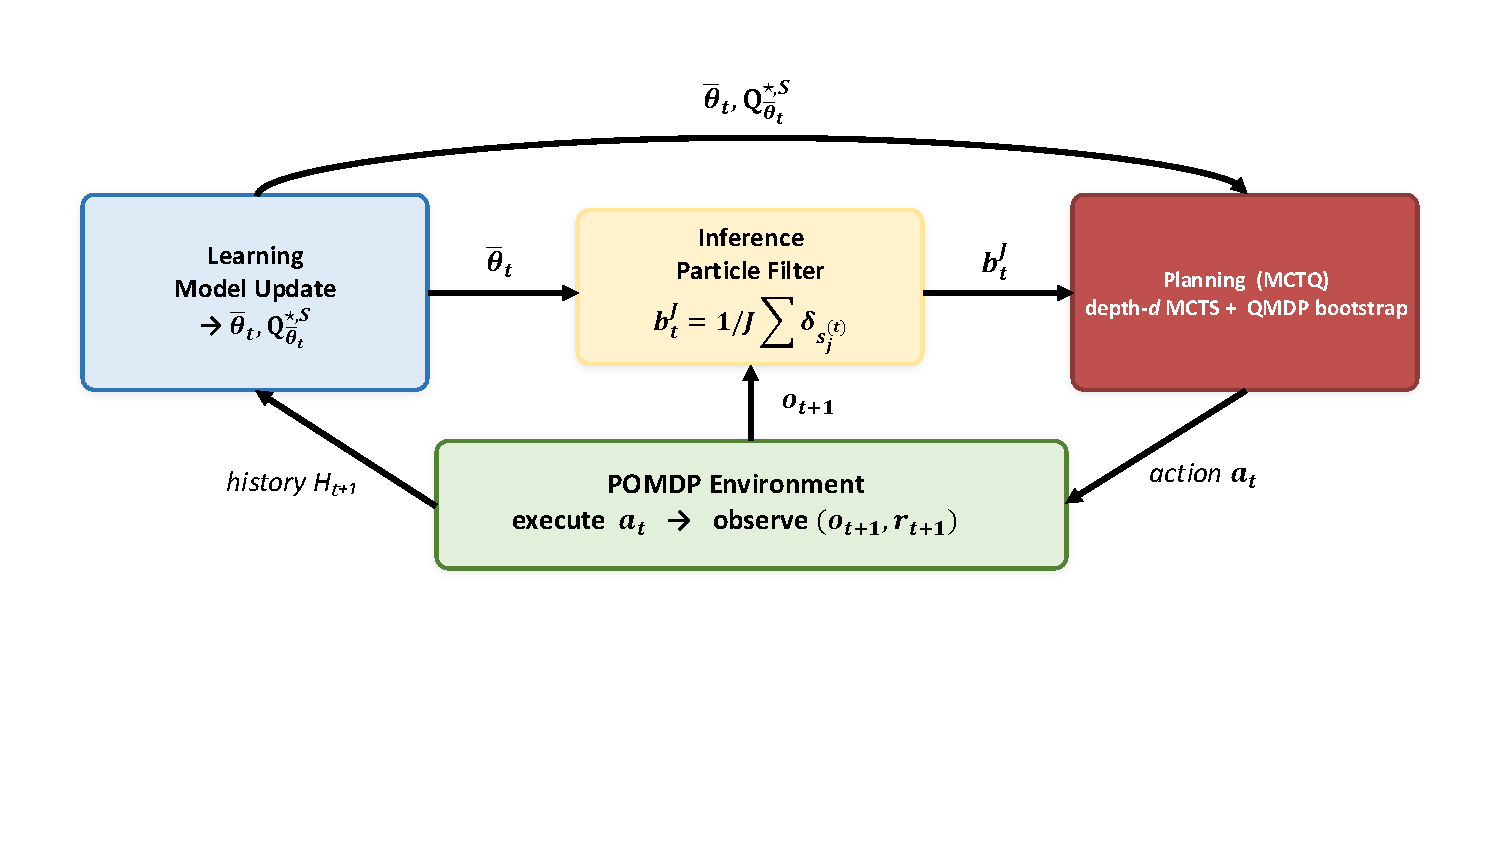
\includegraphics[width=0.8\textwidth]{Figures/pomdp_pipeline.pdf}
%   \vspace{-0.2cm}
%   \caption{The \aigen{Algorithm~\ref{alg:pf_mcts}} online pipeline.}
%   \label{fig:pomdp_pipeline}
% \end{figure}

\begin{algorithm}[t]
\caption[Online particle filtering with finite-depth Monte Carlo belief-tree planning]{\aigen{Online Particle Filtering with Finite-Depth Monte Carlo Belief-Tree Planning.} \aigen{The belief-tree planner} (Algorithm~\ref{alg:mctq}) takes the particle belief $b_t^J$ and returns an estimate $\widehat Q_t(b_t^J,a)$ of $Q_{\bar\theta_k,d}(b_t^J,a)$ for every root action $a\in\gA$.}
\label{alg:pf_mcts}
\begin{algorithmic}[1]
\Require particles $J$; depth $d$; rollouts $N$; horizon $T$; tolerance $\beta$; model class $\Theta$; exploration parameter $\eta>0$.
\State Sample $s^{(1)}_1,\ldots,s^{(1)}_J \sim b_0$.
\State Set epochs $E_k=[2^{k-1},\,2^k)$ for $k=1,\ldots,K:=\lceil\log_2 T\rceil$, with $\varepsilon_k:=\eta/\sqrt{|E_k|}$.
\For{epoch $k=1,2,\ldots,K$}
  \State $\bar\theta_k \gets \textsc{ModelUpdate}(H_{T_k})$ via~\eqref{eq:beta_mle}; compute $\widehat Q^{\mathrm{MDP}}_{\bar\theta_k}\approx Q_{\bar\theta_k}^{\star,S}$.
  \For{$t\in E_k$}
    \State $\{\widehat Q_t(b_t^J,a)\}_{a\in\gA}\gets \textsc{MCTQ}\bigl(\bar\theta_k,\,b_t^J,\,d,\,N,\,\widehat Q^{\mathrm{MDP}}_{\bar\theta_k}\bigr)$ \Comment{Algorithm~\ref{alg:mctq}}
    \State Play $a_t = \arg\max_a \widehat Q_t(b_t^J,a)$ w.p.\ $1-\varepsilon_k$; else $a_t \sim \text{Unif}(\gA)$.
    \State Observe $(o_{t+1},r_t)$.
    \State Propagate, reweight, and resample particles via~\eqref{eq:pf_predict_weight} under $\bar\theta_k$.
  \EndFor
\EndFor
\end{algorithmic}
\end{algorithm}


% \subsection{\aigen{Algorithm~\ref{alg:mctq}}: Monte Carlo tree search with QMDP leaves}
% \label{sec:mctq_planning}


% \aigen{Algorithm~\ref{alg:mctq}} plans on the particle-belief state through a Monte Carlo tree search for the first $d$ steps and averages the fully observable MDP action-values at each leaf node. 
\paragraph{Approximate planning.} For a given current belief, \aigen{Algorithm~\ref{alg:mctq}} runs a Monte Carlo tree search on the belief tree for the first $d$ steps and applies the QMDP approximation at the leaf nodes. This gives a practical middle ground between expensive belief-tree search and the cheap but potentially biased pure QMDP approximation. 


For a belief $b\in\Delta(\gS)$, define the QMDP leaf value and the depth-$d$ belief tree value as 
\begin{equation}
\bar V_{\theta}^{\star,S}(b)
:=
\max_{a\in\gA}\int_{\gS} Q_{\theta}^{\star,S}(s,a)\, b(\mathrm ds), \quad \text{ and } \quad \bar V_{\theta,d}^{\star,S}:=\gT_\theta^d\, \bar V_{\theta}^{\star,S}, \qquad d\ge 0,
\label{eq:U0_def}
\end{equation}
where $Q_{\theta}^{\star,S}$ is the optimal action-value function of the fully observable MDP induced by $\theta$, and $\gT_\theta$ is the Bellman operator of the belief-MDP from~\eqref{eq:bellman_operator}. The corresponding action-value function is defined recursively as
\begin{equation}
Q_{\theta,d}(b,a) := r(b,a)+\gamma \int_{\gO} \bar V_{\theta,d-1}^{\star,S}\bigl(\tau_\theta(b,a,o)\bigr)\, p_\theta(o\mid b,a)\, \mathrm do, \qquad d\ge 1.
\label{eq:Qd_def}
\end{equation}
When $d=0$, $\bar V_{\theta,0}^{\star,S}(b)=\max_a\int Q_\theta^{\star,S}(s,a)\,b(\mathrm ds)$ and \aigen{Algorithm~\ref{alg:mctq}} reduces exactly to QMDP. As $d\to\infty$, $\bar V_{\theta,d}^{\star,S}\to V_\theta^{\star,B}$ (see Proposition~\ref{prop:structural_error} in Appendix~\ref{app:structural_proofs} for the proof).

\paragraph{Particle belief and MCTS approximation.}
In practice, the current belief is represented by a particle approximation $b_t^J=\frac{1}{J}\sum_{j=1}^J \delta_{s_t^{(j)}}$.
Starting from $b^J_t$, \aigen{Algorithm~\ref{alg:mctq}} builds a search tree of depth $d$ with $N$ Monte Carlo simulations per root action, inspired by the POMCP framework~\citep{silver2010monte}.
Each simulation samples a particle from $b_t^J$, descends to depth $d$ using uniform random action selection at internal nodes, expands nodes as it passes through them, and records its state in the particle set $B(v)$ of every node $v$ it visits.
Each depth-$d$ leaf is evaluated by the QMDP value of its pooled particles, $\max_{a'}|B(v)|^{-1}\sum_{s\in B(v)}Q_\theta^{\star,S}(s,a')$, and a bottom-up dynamic program then computes $\widehat Q_t(b_t^J,a)$ for each root action.
Uniform selection is a proof device rather than a performance claim: the analysis only needs the internal rule to read no statistic of the current tree and to give every action probability at least $\pi_{\min}>0$, so a frozen learned proposal also qualifies, whereas UCB1 does not (Appendix~\ref{app:mctq}).

\paragraph{Observation discretization.}
With continuous $\gO$, every simulated observation is distinct, so tree nodes below the root are never revisited and a depth-$d$ tree is not well defined.
\aigen{Algorithm~\ref{alg:mctq}} therefore indexes children by a binned observation $\phi(o)$, where $\phi:\gO\to\bar\gO$ has $M:=|\bar\gO|$ bins of diameter $\mathrm{diam}(\phi)$.
For finite $\gO$ we take $\phi=\mathrm{id}$ and $M=|\gO|$, and for $d=0$ no binning is needed.
The resulting bias and its trade-off against $N$ are made explicit in Theorem~\ref{thm:final_regret_bound}.
% : at each leaf, the QMDP value of accumulated particles; at each internal node, $\hat V(v)=\max_{a'}\hat Q(v,a')$ where $\hat Q(v,a')$ is the empirical mean return for action $a'$. The root statistics provide the estimates $\widehat Q_t(b_t^J,a)\approx Q_{\theta,d}(b_t^J,a)$, and the agent selects $\hat a_t\in\arg\max_{a}\widehat Q_t(b_t^J,a)$. The full pseudocode is given in Algorithms~\ref{alg:mctq}--\ref{alg:simulate} in Appendix~\ref{app:mctq}.


\section{Error Analysis and Regret Guarantee}
\label{sec:analysis}


We measure performance by the expected cumulative regret defined as:
\begin{equation}\label{eq:regret_def_sec4}
\mathrm{Reg}_T := \E\!\left[\sum_{t=1}^T \text{regret}_t \right] :=\E\!\left[\sum_{t=1}^T\bigl(V_{\theta^\star}^{\star,B}(b_t)-V_{\theta^\star}^{\pi_t,B}(b_t)\bigr)\right],
\end{equation}
where $\pi_t$ is the policy deployed from round $t$, and the expectation is over the trajectory and algorithmic randomness. A key contribution is an end-to-end regret bound for \aigen{Algorithm~\ref{alg:pf_mcts}}, enabled by the following novel regret decomposition. Let $k(t)$ denote the epoch containing round $t$, and $\bar\theta_{k(t)}$ be the frozen model during that epoch:
\begin{align}
\text{regret}_t
=
\underbrace{V_{\theta^\star}^{\star,B}(b_t)-V_{\bar\theta_{k(t)}}^{\star,B}(b_t)}_{\text{(A) optimal-value model error}}
+
\underbrace{V_{\bar\theta_{k(t)}}^{\star,B}(b_t)-V_{\bar\theta_{k(t)}}^{\pi_t,B}(b_t)}_{\text{(B) planning + state-id error}}
+
\underbrace{V_{\bar\theta_{k(t)}}^{\pi_t,B}(b_t)-V_{\theta^\star}^{\pi_t,B}(b_t)}_{\text{(C) fixed-policy model error}}, \label{eq:main_decomp_round_t}
\end{align}
Terms (A) and (C) capture model estimation error: the gap between $\bar\theta_{k(t)}$ and $\theta^\star$. Term (B) captures planning approximation under the learned model, which is further decomposed into three sources:
\begin{equation}
 \text{(B)} \;\le\;
\underbrace{\bigl|V_{\bar\theta_{k(t)}}^{\star,B}(b_t)-V_{\bar\theta_{k(t)}}^{\star,B}(b_t^J)\bigr|}_{\text{(B1) belief approx.}}
+
\underbrace{V_{\bar\theta_{k(t)}}^{\star,B}(b_t^J)-V_{\bar\theta_{k(t)}}^{\pi_t,B}(b_t^J)}_{\text{(B2) planning suboptimality}}
+
\underbrace{\bigl|V_{\bar\theta_{k(t)}}^{\pi_t,B}(b_t^J)-V_{\bar \theta_{k(t)}}^{\pi_t,B}(b_t)\bigr|}_{\text{(B1$'$) belief approx.}}. \label{eq:B_decomp}
\end{equation}
Terms (B1) and (B1$'$) measure the cost of evaluating value functions at the particle belief $b_t^J$ instead of the true posterior $b_t$, each bounded by $O(1/J^{1/(2\kappa_{\mathrm{pf}})})$ via particle-filter concentration.
The planning gap (B2) further splits into Monte Carlo error from finite MCTS rollouts ($O(1/\sqrt{N})$) and structural error from QMDP bootstrapping at depth $d$.

\textbf{Three objects.} The analysis separates the belief-MDP optimum $V_\theta^{\star,B}$, the deterministic \emph{planning target} $\bar V_{\theta,d}^{\star,S}=\gT_\theta^d\bar V_\theta^{\star,S}$ of~\eqref{eq:U0_def}, and the randomized estimate $\widehat Q_t(b_t^J,a)$ that \aigen{Algorithm~\ref{alg:mctq}} computes from pooled particle sets.
The target differs from the optimum by the structural error, which decays geometrically in $d$ and involves no particles, whereas the estimate differs from the target by the Monte Carlo error, which grows with $d$, so for a fixed $N$ the bound is U-shaped in the depth.
Each component enters only through an interface (a $\beta$-approximate MLE oracle, an SMC filter with an $L^p$ bound, a planner with a Monte Carlo error bound), so the decomposition survives substituting, e.g., POMCP-style planners or variational filters.


% Terms (A) and (C) capture model estimation error: the gap between the learned model $\bar\theta_t$ and the true model $\theta^\star$. Term (B) captures the planning approximation under the learned model, which further decomposes into three sources: (i) Monte Carlo error from finite MCTS rollouts, (ii) structural error from QMDP bootstrapping at depth $d$, and (iii) particle-belief approximation error from representing $b_t$ by a finite particle set $b_t^J$. 

% \paragraph{Structural error and the Jensen gap.}


\subsection{Assumptions and main result}
\label{sec:final_regret}

Modern SMC analyses \citep{delMoral04, chopin20, karjalainen23} impose rather unavoidable but stringent conditions on the transition kernel and observation density. We inherit these in the form of the following Doeblin and bounded observation density assumption (Assumption \ref{aspt:particle_error}) on the latent dynamics. This choice aligns well with our aim to provide an end-to-end regret bound that decomposes error across the learning--inference--planning pipeline, interpolating between theory and practice, rather than to develop optimal exploration methods for POMDP model estimation, as Assumption \ref{aspt:particle_error} ensures that simple exploration strategies like $\varepsilon$-greedy have sufficient coverage. At the same time, the Doeblin condition resembles commonplace strong mixing assumptions within the RL literature \citep{gaur2024closing, wu2022finitetimeanalysistimescale, xu2020improving, kausik2023learning} and the $\alpha$-revealing condition commonplace in the POMDP literature plays a similar role to the bounded observation density condition \citep{liu2022partially,liu2023optimistic}.

% This assumption is standard in the sequential Monte Carlo literature: the Doeblin condition and bounded weights are the canonical conditions for time-uniform stability of particle filters and Feynman-Kac particle systems~\cite{delMoral04, crisan2002survey, whiteley2013stability, doucmoulinesolsson2014, chopin2004central}. 
% While strong from an RL perspective---it ensures passive state coverage and precludes the need for strategic state-space exploration---the Doeblin condition does \emph{not} provide coverage over the action space. 
% To be clear, this assumption is commonplace in the SMC literature, to the point where it is rather unavoidable within modern analyses \cite{delMoral04, chopin20}. At the same time, the Doeblin condition resembles commonplace strong mixing assumptions within the RL literature \citep{gaur2024closing, wu2022finitetimeanalysistimescale, xu2020improving, kausik2023learning} and the $\alpha$-revealing condition commonplace in the POMDP literature is spiritually similar to the bounded observation density condition \citep{liu2022partially,liu2023optimistic}.

\begin{aspt}[Uniform mixing and bounded weights]\label{aspt:particle_error} \text{ }
\begin{enumerate}
\item \emph{Uniform Doeblin condition.} There exist $\varepsilon_{\mathrm{mix}}>0$ and a probability measure $\nu\in\Delta(\gS)$ such that $P_\theta(\cdot\mid s,a)\ge \varepsilon_{\mathrm{mix}}\,\nu(\cdot)$ for all $(\theta,s,a)\in\Theta\times\gS\times\gA$.
\item \emph{Bounded observation density.} There exist $0<g_{\min}\le g_{\max}<\infty$ such that $g_{\min}\le Z_\theta(o\mid s)\le g_{\max}$ for all $(\theta,s,o)\in\Theta\times\gS\times\gO$.
\end{enumerate}
\end{aspt}

% \ziping{talk about some naive bound one can have about these parameters.}


% \kevin{We're not trying to get an optimal bound, we want to decompose the error into different sources and control them separately for end-to-end regret guarantees for practical algorithms. The missing gap in the literature is that end to end regret is only for computationally intractable theory algorithms. We identify tradeoffs and approximations to interpolate between theory and practice.}


% A significant technical contribution is that Assumption \ref{aspt:particle_error} guarantees that $\varepsilon_t$-greedy exploration provides sufficient support over action and state pairs. This support is needed to transfer the MLE concentration of the history policies to the current policy and to achieve sublinear regret for model estimation. \kevin{Move to technical contributions subsection.}

% \ziping{Say that we could do $\epsilon_t$ scheduling to achieve the $\sqrt{T}$. This is non-trivial from the literature.}

Let $\gN_\Theta(\varepsilon)$ denote the $\varepsilon$-covering number of $\Theta$, i.e.\ the minimum number of $\ell_1$-balls of radius $\varepsilon$ (in the metric defined as trajectory level likelihood) needed to cover $\Theta$. Define the effective model complexity $\beta_T:=\beta+\log\bigl[\gN_\Theta(1/T)\,T/\delta\bigr]$, where $\beta$ is the MLE tolerance from~\eqref{eq:beta_mle} and $\delta\in(0,1)$ is a confidence parameter.

\begin{thm}[End-to-end regret of \aigen{Algorithm~\ref{alg:pf_mcts}}]\label{thm:final_regret_bound}
Suppose Assumption~\ref{aspt:particle_error} holds. Algorithm~\ref{alg:pf_mcts}, run with exploration parameter $\eta\asymp T^{1/4}(\beta_T/\log T)^{1/4}$ and observation binning $\phi$ with $M$ bins of diameter $\mathrm{diam}(\phi)=\omega_Z^{-1}\bigl((1-\gamma)g_{\min}/(2\gamma g_{\max}V_{\max}\sqrt N)\bigr)$ ($\phi=\mathrm{id}$ and $M=|\gO|$ when $\gO$ is finite), and, if $d\ge2$, $N$ above the threshold of Remark~\ref{rmk:mc_constants}, and $\kappa_{\mathrm{pf}}:=\max \left(1, {\log \left(2 g_{\max }^2 / g_{\min }^2\right)}/{\log (1 / \gamma)}\right)$ satisfies
% $\eta=\Theta(K_{\mathrm{cov}}^{1/2}\,T^{1/4}(\beta_T/\log T)^{1/4})$ where $K_{\mathrm{cov}}:=H|\gA|\,g_{\max}^2/(\varepsilon_{\mathrm{mix}}\,g_{\min}^2)$, for any depth $d\ge 0$,
\begin{align}
\mathrm{Reg}_T
\;\le\;
\underbrace{\widetilde O\!\left(\frac{C_{\mathrm{est}}\, R_{\max}}{(1-\gamma)^{3/2}}\,T^{3/4}\right)}_{\text{model + exploration + filter}}
+
\underbrace{\frac{C_{\mathrm{pf}}\,R_{\max}}{(1-\gamma)^2}\cdot\frac{T}{J^{1/(2\kappa_{\mathrm{pf}})}}}_{\text{particle approx.}}
 +
\underbrace{\frac{C_{\mathrm{mc}}\,R_{\max}}{(1-\gamma)^2}\cdot\frac{T}{\sqrt{N}}}_{\text{Monte Carlo}}
+
\underbrace{\frac{2\gamma^{d+1}}{(1-\gamma)^2}\sum_{t=1}^T\Xi_{\bar{\theta}_{k(t)}}}_{\text{QMDP structural bias}}, \nonumber
% \label{eq:final_regret_bound}  
\end{align}
\end{thm}
Here $\widetilde O$ hides factors polylogarithmic in $T$, $\omega_Z$ is the modulus of continuity of the observation likelihood ratio (Appendix~\ref{app:planning_state_proofs}), $M=|\bar\gO|$ is the number of observation bins, and $\Xi_{\bar{\theta}_{k(t)}}$ is the QMDP structural bias of~\eqref{eq:Xi_def}.
The coefficients are
\begin{align*}
    C_{\mathrm{est}} &= \mathrm{Poly}(|\gA|, g_{\max}/g_{\min}, \epsilon_\mathrm{mix}^{-1}, \log(1/\gamma), \log\gN_\Theta(1/T), \beta), \quad C_{\mathrm{mc}} = \textstyle{O(d\gamma^d  |\gA|^{(d+3)/2}M^{d/2})},\\
    C_{\mathrm{pf}} &=\widetilde{O}\bigl(V_{\max}^2\,g_{\max}/(\varepsilon_{\mathrm{mix}}^3\,g_{\min})\cdot(\log J)^{3/2}\sqrt{\log(\gN_\Theta(1/T)\,|\gA|)}\bigr) \;\; \text{ (See ~\eqref{eq:Cpf_explicit})}.
\end{align*}


% where the $\widetilde{O}$ absorbs factors polylogarithmic in $T$; $C_{\mathrm{est}}$ depends polynomially on $|\gA|$, $g_{\max}/g_{\min}$, $1/\varepsilon_{\mathrm{mix}}$, $\gN_\Theta(1/T)$, $\beta$, and $\log(1/\gamma)$; $C_{\mathrm{pf}}'=c_H\,V_{\max}(g_{\max}/g_{\min})^{2H}/\varepsilon_{\mathrm{mix}}^3\cdot\sqrt{\log(\gN_\Theta(1/T)\,|\gA|^H)}$ with $H=\lceil\log(4V_{\max}\sqrt{J})/\log(1/\gamma)\rceil$ and $c_H$ polynomial in $H$; $C_{\mathrm{mc}}:=2\sqrt{2|\gA|}\,(1+c_0\,\Phi_d\sqrt{|\gA|})$ with $c_0>0$ a universal constant (from Hoeffding's inequality applied under uniform exploration) and $\Phi_d=\sum_{k=1}^{d-1}(\gamma\sqrt{|\gA|M})^k$, where $M=|\bar\gO|$ is the number of observation discretization bins; and $\Xi_{\bar{\theta}_{k(t)}}$ captures the QMDP structural bias.

\textbf{Reading the bound.} Theorem \ref{thm:final_regret_bound} bounds cumulative regret with four major terms. The first term captures model estimation error, exploration cost, and filter mismatch between the true posterior $b_t^{\theta^{\star}}$ and the particle belief $b_t^{\bar\theta_{1:K}}$. The $\widetilde O(T^{3/4})$ rate arises from the coverage transfer needed to bound the optimal-value model error (term~(A) in~\eqref{eq:main_decomp_round_t}) via $\varepsilon$-greedy exploration. Terms 2, 3, and 4 capture the total approximate planning errors that may scale linearly in $T$. They can be diminished by increasing the number of particles $J$, number of Monte Carlo rollouts $N$, and the planning depth $d$.
The particle error decays as $J^{-1/(2\kappa_{\mathrm{pf}})}$ at cost $O(J)$, the Monte Carlo error as $N^{-1/2}$ at cost $O(N)$, and the structural error as $\gamma^{d}$ at a tree size of up to $(|\gA|M)^{d}$ nodes.
The bound therefore exposes a \textbf{sample-vs.-computational efficiency trade-off} through the marginal return of each budget, but a concrete allocation requires knowledge of $\kappa_{\mathrm{pf}}$ and $\Xi_\theta$ and is not an optimality statement.
\aigen{Section~\ref{sec:validation} empirically validates each of these four scaling laws on a Doeblin-mixing POMDP satisfying Assumption~\ref{aspt:particle_error} and demonstrates how the decomposition guides the choice of $(J, N, d)$ under a target per-term error tolerance.}
With continuous observations, the binning keeps the discretization bias at the Monte Carlo order $O(V_{\max}/\sqrt N)$, and the price is paid in the constant: $M$ grows as $N^{d_o/2}$ for $\gO\subseteq\R^{d_o}$, so $C_{\mathrm{mc}}$ grows exponentially in $d\cdot d_o$, whereas balancing bin width against $N$ instead gives the rate $\widetilde O(N^{-1/(d\,d_o+2)})$ (Remark~\ref{rmk:disc_resolution}).
This cost is absent only at $d=0$, the regime used in our deep RL experiments.

\textbf{Technical challenges.} Bounding each source in~\eqref{eq:B_decomp} under online learning raises three difficulties. First, controlling (B1) requires working with a test-function class defined directly over $\gS$, rather than only the parametric family $\{Q^{\star,B}_\theta\}_\theta$. This is because the belief-space value functions may lack the regularity needed for uniform particle-filter error control. In fact, the planning-induced class over multiple steps is effectively uncountable over the possible model parameters, so we control it through truncation. The required truncation level depends on the desired particle approximation accuracy: as the particle error target decreases, the tail must be made smaller, which enlarges the truncated function class. This creates a tradeoff between the complexity of the truncated class and the particle ensemble size, leading to a slower ($1/J^{1/2\kappa_{\mathrm{pf}}}$), essentially nonparametric, rate that emphasizes the technical challenge of the problem.

Second, the filtering analysis must account for the fact that the data are generated online by a changing policy. Classical particle-filter stability assumes a fixed generative model, whereas here the filter receives actions from a non-stationary, improving policy. We extend time-uniform $L^p$ bounds~\citep{delMoral04} to this setting by exploiting the Doeblin condition uniformly over actions. Third, since Doeblin coverage applies only to states and not actions, we further ensure action coverage via $\varepsilon$-greedy exploration. This enables us to transfer the MLE concentration result across policies, controlling both terms (A) and (C), and to control the Monte Carlo error in (B2).

\begin{rmk}[Where the hardness of POMDPs goes]
POMDP sample complexity may in the worst case scale exponentially in the effective horizon $1/(1-\gamma)$.
Our bound is polynomial in $1/(1-\gamma)$ for two reasons.
First, under the Doeblin condition the Bayes filter forgets its initialization at a geometric rate $\rho=1-\varepsilon_{\mathrm{mix}}g_{\min}/g_{\max}<1$ uniformly over actions, so errors add up over time rather than compound.
Second, bounded observation densities play the role of the $\alpha$-revealing condition~\citep{liu2022partially}: they bound importance weights, so data transfer across policies without an $(|\gA|/\varepsilon)^{H}$ blow-up, and particle weights stay non-degenerate.
This does not circumvent the lower bound: $\varepsilon_{\mathrm{mix}}^{-1}$ and $g_{\max}/g_{\min}$ can be exponential in the effective horizon for hard instances, and $C_{\mathrm{est}}$ and $C_{\mathrm{pf}}$ depend polynomially on them.
\aigen{Appendix~\ref{sec:app08-stress-tests} provides controlled stress tests illustrating the mechanisms by which violations of $g_{\min}>0$ and large multi-step information-gathering gaps $\Xi(\theta_\star)$ affect filtering and shallow planning.}
\end{rmk}

\begin{rmk}[Bypassing exploration with offline coverage]
The $\widetilde O(T^{3/4})$ rate is driven by the coverage transfer for term~(A), which requires $\varepsilon$-greedy exploration to ensure model accuracy at the optimal policy. If instead the agent has access to $N_{\mathrm{off}}$ offline trajectories from a behavior policy $\pi_b$ with single-policy concentrability $c_{\mathrm{off}}^\star$ (the worst-case ratio of trajectory $\ell_1$ distances between $\pi^\star$ and $\pi_b$), then greedy exploitation ($\varepsilon_t=0$) achieves regret $\widetilde O(\sqrt{T}/(1-\gamma)) + O(c_{\mathrm{off}}^\star T/(\sqrt{N_{\mathrm{off}}}(1-\gamma)))$ plus computational terms. When $N_{\mathrm{off}} \ge (c_{\mathrm{off}}^\star)^2 T$, the total regret is $\widetilde O(\sqrt{T})$ without any additional online exploration. The formal statement and proof are in Appendix~\ref{app:offline_coverage}.
\end{rmk}

% \ziping{Say that in the worst case $gmax / gmin$ or $1/\epsilon_{mix}$ can be exponential in $1/\gamma$. Analyses like PS4POMDP have explicit $H$ exponential dependence. Our bounds are instance-dependent in general, but this dependence can indeed be there in the worst-case.}


% \kevin{We know that POMDPs in general have exponential in $H$ dependence, and the particle filter has exponential dependence in the dimension of the state space in general. How does this relate to our result?}

 
% \begin{equation}\label{eq:C_est_def}
% C_{\mathrm{est}}:=4\sqrt{C_{\mathrm{model}}},
% \qquad
% C_{\mathrm{model}}:=C_0\cdot\frac{H\,|\gA|\,g_{\max}^2}{\varepsilon_{\mathrm{mix}}\,g_{\min}^2},
% \qquad
% C_0:=4\sqrt{c}\bigl(1+C_{\mathrm{filt}}/(1-\rho)\bigr),
% \end{equation}
% with $C_{\mathrm{filt}}:=g_{\max}/g_{\min}$, $\rho:=1-\varepsilon_{\mathrm{mix}}\,g_{\min}/g_{\max}$, $c$ the universal constant from Proposition~\ref{prop:lik_to_l1}, and $H=O(\log T/\log(1/\gamma))$.

% The exact form of $C_{\mathrm{est}}$, the optimal exploration schedule, and the proof are given in Appendix~\ref{app:regret_proof} and \ref{app:exploration_schedule}. The first term consolidates model estimation, exploration cost, and filter mismatch into a single $\widetilde O(\sqrt{T})$ term (the $(\beta_T/\log T)^{1/4}$ factor is $O(1)$ since $\beta_T=O(\log T)$). This is achieved by setting $\varepsilon_t= \Theta(t^{-1/2})$. The constant $C_{\mathrm{est}}\propto \sqrt{H\,|\gA|}$ from the Doeblin mixing condition, which avoids the exponential $(|\gA|/\varepsilon)^H$ blowup of a naive propensity-score argument.

% The remaining terms shrink with the computational resources $J,N$ and the search depth $d$.
% The structural term is controlled by $\Xi_t$. The case studies below show that the QMDP \emph{policy} is optimal in the LQG setting (the Jensen gap $\Xi_\theta=\tr((M-P)\bar\Sigma)$ is zero only when $\Gamma=0$, but the QMDP action coincides with the belief-MDP optimal action for all $\Gamma$ by the separation principle), and that $\Xi_t$ vanishes at rate $\rho_t$ in the identifiable contextual MDP.


\subsection{Understanding the structural bias}
\label{sec:understanding_structural_bias}

It remains to discuss the QMDP approximation error, which is governed by the \emph{Jensen gap}
\begin{equation}
\Xi_\theta
:=
\sup_{b\in\Delta(\gS)}
\left(
\int_{\gS}V_\theta^{\star,S}(s)\,b(\mathrm ds)
-
\max_{a\in\gA}\int_{\gS}Q_\theta^{\star,S}(s,a)\,b(\mathrm ds)
\right),
\label{eq:Xi_def}
\end{equation}
which measures the value lost by choosing a single action for all states (QMDP planning) rather than the state-dependent optimal action. We show (Proposition~\ref{prop:structural_error} in Appendix~\ref{app:structural_proofs}) that the depth-$d$ belief-tree structural error of \aigen{Algorithm~\ref{alg:mctq}} satisfies $\|\bar V_{\theta,d}^{\star,S}-V_{\theta}^{\star,B}\|_\infty\le\frac{\gamma^{d+1}}{1-\gamma}\Xi_\theta$, decaying geometrically with depth $d$.

The structural quantity $\Xi_\theta$ admits a natural interpretation in terms of posterior \emph{variance} of value-relevant features. Let $g:\gS\to\R^k$ be a measurable embedding, and write
$m_g(b):=\E_{S\sim b}[g(S)]$ and $\Sigma_g(b):=\Cov_{S\sim b}(g(S))$.

\begin{aspt}[Value-relevant embedding]\label{aspt:value_embedding_main}
There exist twice continuously differentiable maps $F_\theta^a:\R^k\to\R$ for each $a\in\gA$ such that
$Q_\theta^{\star,S}(s,a)=F_\theta^a(g(s))$ for all $(s,a)\in\gS\times\gA$, with curvature bounds, where $F_\theta(x):=\max_a F_\theta^a(x)$ and $V_\theta^{\star,S}(s)=F_\theta(g(s))$, of
\[
\sup_{a\in\gA}\sup_{x\in\mathrm{conv}(g(\gS))}\bigl\|\nabla^2 F_\theta^a(x)\bigr\|_{\mathrm{op}}\le L_\theta
\qquad\text{and}\qquad
\sup_{x\in\mathrm{conv}(g(\gS))}\bigl\|\nabla^2 F_\theta(x)\bigr\|_{\mathrm{op}}\le L_\theta
,\]
where $\|\cdot\|_{\mathrm{op}}$ is the spectral norm.
\end{aspt}
% The second curvature condition on $F_\theta=\max_a F_\theta^a$ is a genuine assumption: while $\max$ of finitely many $C^2$ functions is $C^2$ away from the switching boundaries where the maximizing action changes, $F_\theta$ is generally \emph{not} twice differentiable on those boundaries. However, the bound in Proposition~\ref{prop:variance_qmdp_bias_main} only requires curvature control on each $F_\theta^a$ individually (for the lower bound on $\bar V_\theta^{\star,S}$) and on $F_\theta$ (for the upper bound on $\widetilde V_\theta^{\star}$). 
In practice, the condition holds when either (i) a single action is optimal throughout $\mathrm{conv}(g(\gS))$, or (ii) $F_\theta$ is a single smooth function of $s$ (as in linear-quadratic-Gaussian (LQG) systems, where it is a quadratic form and both conditions hold with the same $L_\theta$).

\begin{prop}[Curvature bound on $\Xi_\theta$]\label{prop:variance_qmdp_bias_main}
Under Assumption~\ref{aspt:value_embedding_main}, for every belief $b\in\Delta(\gS)$,
\begin{equation}
\Xi_\theta(b)
:=\widetilde V_\theta^{\star}(b)-\bar V_\theta^{\star,S}(b) 
\;\le\;
L_\theta\,\tr\bigl(\Sigma_g(b)\bigr), 
\label{eq:variance_xi_bound_main}
\end{equation}
where $\widetilde V_\theta^{\star}(b):=\int_{\gS}V_\theta^{\star,S}(s)\,b(\mathrm ds)$ is the linear QMDP surrogate.
In particular, $\Xi_\theta=\sup_b\Xi_\theta(b)$.
\end{prop}

The proof is given in Appendix~\ref{app:variance_proofs}.
That QMDP is accurate once the belief concentrates is expected; Proposition~\ref{prop:variance_qmdp_bias_main} is sharper in two ways.
First, only the posterior covariance of the value-relevant features $g$ matters, so uncertainty in directions to which the value is insensitive costs nothing and concentration of the full belief is not necessary.
Second, the curvature $L_\theta$ converts this covariance into a value gap, which then enters Theorem~\ref{thm:final_regret_bound} as $\gamma^{d+1}\Xi_\theta/(1-\gamma)$ and is traded off against planning depth.
In discounted LQG, for instance, the Kalman covariance converges to a strictly positive steady state and never vanishes, yet the QMDP policy is belief-optimal, and $\Xi_\theta=0$ when the control does not enter the dynamics (Appendix~\ref{app:case_study_proofs}).
% Combined with Proposition~\ref{prop:structural_error}, the total \aigen{Algorithm~\ref{alg:mctq}} error is
% $\|\bar V_{\theta,d}^{\star,S}-V_\theta^{\star,B}\|_\infty\le\frac{\gamma^{d+1}}{1-\gamma}L_\theta\sup_b\tr(\Sigma_g(b))$, which decays geometrically with depth $d$.

% \paragraph{Case studies.}
% \ziping{Cut the case studies a bit more to save space.} \ziping{Give a bit more intuition.}
Appendix~\ref{app:case_study_proofs} instantiates the structural analysis on linear-quadratic Gaussian systems, where $\Xi_\theta$ has a closed form in terms of the Riccati solution and the steady-state Kalman covariance, and on contextual MDPs with identifiable latent context, where $\Xi_{\theta,t}\le 2V_{\max}\rho_t$ for a context-misidentification probability $\rho_t$, which turns ``eventually identified'' into the rate condition $\sum_t\rho_t=o(\sqrt T)$.
% For each, we bound $\Xi_\theta$ and the QMDP policy suboptimality $\sup_b[V_\theta^{\star,B}(b)-V_\theta^{\pi_{\mathrm{Q}},B}(b)]$, where $\pi_{\mathrm{Q}}(b):=\arg\max_a\int Q_\theta^{\star,S}(s,a)\,b(\mathrm ds)$ is the QMDP policy. Proofs are in Appendix~\ref{app:case_study_proofs}.

% \textbf{Case 1: Discounted partially observed LQG.}
% Consider linear-Gaussian dynamics
% $S_{t+1}=\Phi S_t+\Gamma A_t+W_t$, $O_t=H S_t+\eta_t$,
% with $W_t\sim\gN(0,\Sigma_W)$, $\eta_t\sim\gN(0,\Sigma_\eta)$ i.i.d., quadratic reward $r(s,a)=-(s^\top Q_{\mathrm{c}} s+a^\top Ra)$, $Q_{\mathrm{c}}\succeq 0$, $R\succ 0$. Assume $(\Phi,\Gamma)$ is stabilizable and $(\Phi,H)$ is detectable. For LQG, we obtain the closed-form expression $\Xi_\theta =\tr\bigl((M-P)\,\bar\Sigma\bigr)$, where $P$ solve the Riccati equation, $M = Q_c + \gamma \Phi^{\top} P \Phi$, and $\bar \Sigma$ is the steady-state Kalman predictive covariance. When $\Gamma = 0$, we have $M = P$ and $\Xi_{\theta} = 0$. Note that for LQG, the QMDP policy is always optimal.

% \begin{cor}[LQG]\label{cor:lqg}
% Let $M:=Q_{\mathrm{c}}+\gamma\Phi^\top P\Phi$ where $P\succeq 0$ solves the discounted algebraic Riccati equation, and let $\bar\Sigma_{\mathrm{post}}$ be the steady-state Kalman posterior (filtered) covariance satisfying $\bar\Sigma_{\mathrm{post}}=\bar\Sigma - \bar\Sigma H^\top(H\bar\Sigma H^\top+\Sigma_\eta)^{-1}H\bar\Sigma$ with $\bar\Sigma:=\Phi\bar\Sigma_{\mathrm{post}}\Phi^\top+\Sigma_W$ the steady-state predictive covariance. Then
% $\Xi_\theta =\tr\bigl((M-P)\,\bar\Sigma\bigr)$ and the QMDP policy is belief-MDP optimal: $\sup_b\bigl[V_\theta^{\star,B}(b)-V_\theta^{\pi_{\mathrm{Q}},B}(b)\bigr]=0$.
% \end{cor}

% The QMDP action equals the certainty-equivalent LQR control $a=Km$, which is belief-MDP optimal by the separation principle.
% When $\Gamma=0$, the gives $M=P$, so $\Xi_\theta=0$: the QMDP value and the belief-MDP value coincide exactly. When $\Gamma\neq 0$, $M-P\succeq 0$ is generically nonzero, so $\Xi_\theta>0$; the QMDP \emph{policy} remains optimal, but the QMDP \emph{value} underestimates the belief-MDP value by $\tr((M-P)\bar\Sigma)$.

% \emph{Remark.} LQG has unbounded reward and $V_{\max}=\infty$, so it lies outside the standing assumption $|r(s,a)|\le R_{\max}$ of Theorem~\ref{thm:final_regret_bound}. The corollary illustrates the structural analysis (Jensen gap and policy optimality) but does not directly instantiate the regret bound.

% \textbf{Case 2: Identifiable contextual MDP.}
% Consider an episodic contextual MDP \cite{kausik2023learning} with a fixed latent context $C\in\gC$ sampled once per episode and Markov dynamics $S_{t+1}\sim P_c(\cdot\mid S_t,A_t)$, $r_t=r_c(S_t,A_t)$ given $C=c$. Assume
% (i) there exists an estimator $\widehat C_t=\widehat C_t(H_t)$ with $\PP(\widehat C_t\neq C)\le \rho_t$, $\rho_t\downarrow 0$; and
% (ii) $\sup_{c\in\gC}\|V_c^{\star,S}\|_\infty\le V_{\max}$.
% Then $\Xi_{\theta,t}\;\le\; 2V_{\max}\,\rho_t$ and $\sup_b\bigl[V_\theta^{\star,B}(b)-V_\theta^{\pi_{\mathrm{Q}},B}(b)\bigr]\;\le\;{4\gamma\, V_{\max}}\,\rho_t/{(1-\gamma)^2}$. As the context becomes identifiable ($\rho_t\to 0$), both the structural residual and the QMDP policy suboptimality vanish. For the structural bias term $\sum_t\Xi_t\le 2V_{\max}\sum_t\rho_t$ to be $o(\sqrt{T})$, we need $\sum_{t=1}^T\rho_t=o(\sqrt{T})$. 
% This result also suggests a schedule for the planning depth d that decays with $t$, reflecting diminishing structural bias.

\section{Experiments}
\label{ch08:sec:experiments}


\begin{figure}[t]
    \centering
    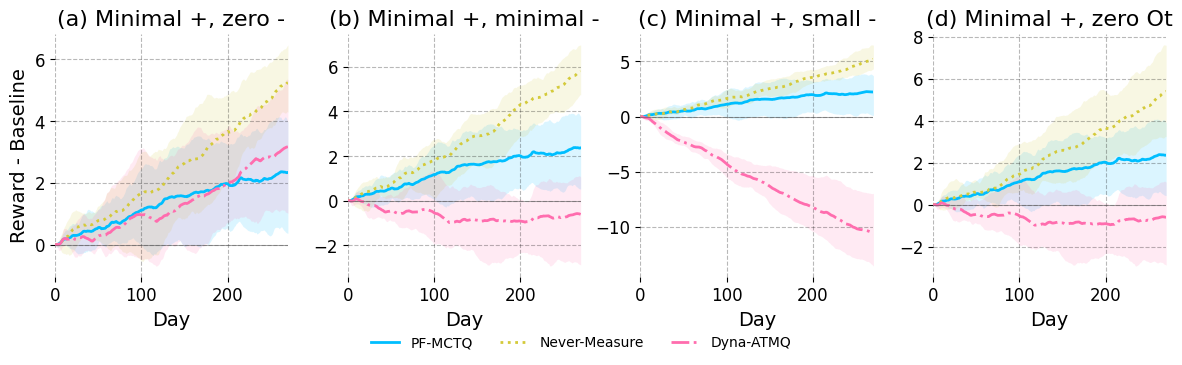
\includegraphics[width=\linewidth]{figures/ch08/Figures/heartsteps.png}
    \vspace{-4ex}
    \caption[Cumulative reward above baseline across four HeartSteps scenarios]{Cumulative reward above the baseline rollout across four HeartSteps scenarios, where the positive intervention effect and the delayed negative measurement effect or proxy $O_t$ informativeness are varied. Mean and 2.5\% and 97.5\% quantiles displayed on five seeds.}
    \label{fig:heartsteps}
\end{figure}


% \kevin{Objective is not to get the best policy in general, it is to do as well as possible with limited samples. }

% \kevin{we use the pypomp package and mop/vsmc gradient estimates, and plan via particle rollouts. we also employ an actor and a critic, essentially instantiating this as particle filtering and model-based planning on top of recurrent SAC.}

% \kevin{This is not intended to get you state-of-the-art performance. Rather, it is intended as a proof of concept to show that particle-based filtering and planning can be implemented on top of existing deep RL algorithms without too much overhead. In doing so, we use highly optimized JAX implementations of the particle filter on GPU. }

% \kevin{The biggest gap from the theory is that we use rollout planning (of each particle) instead of particle belief planning within the experiments, to further reduce the computational burden. We anticipate that results will improve with particle belief planning. See Appendix for analysis of the gap between particle belief and rollout planning. This is the gap between the POMDP value of the QMDP policy and the true optimal value of the POMDP.}


% \ziping{Mojoco environment, heartstep environment, LQR (talking about particle posterior diagnosis, emphesize state identifiability).}


Our experiments test whether particle filtering and model-based planning can be used as a practical layer on top of modern deep reinforcement learning under partial observability.
Here, our goal is not to obtain state-of-the-art asymptotic performance.
Instead, we aim to evaluate whether explicit particle beliefs can improve low-sample decision making with modest additional machinery.
Table~\ref{tab:theory_coverage} states which experiments fall under the theory: the deep RL experiments demonstrate that the pipeline is practical and are not evidence for the constants of Theorem~\ref{thm:final_regret_bound}.

\begin{aigenblock}
\subsection{Empirical Validation of the Regret Decomposition}
\label{sec:validation}

To verify the individual scaling rates predicted by Theorem~\ref{thm:final_regret_bound} in an environment where all theoretical assumptions hold with known constants, we evaluate Algorithm~\ref{alg:pf_mcts} on a Doeblin-mixing modification of the Tiger POMDP (listening transition $0.95\BI + 0.05\BU$, uniform reset upon opening, rewards scaled to $[0,1]$, $\varepsilon_{\mathrm{mix}} = 0.05$, $0.15 \leq Z \leq 0.85$, and discount factor $\gamma = 0.80$). Figure~\ref{fig:theory_bound_audit} and Table~\ref{tab:fitted_rates} report the empirical decay of each isolated error term in the regret decomposition as we sweep the particle count $J \in \{8,\dots,512\}$, the rollout count $N \in \{4,\dots,512\}$, the belief-tree depth $d \in \{0,\dots,12\}$, and the online trajectory count $T$. Each empirical slope closely tracks its theoretical counterpart. Moreover, evaluating the isolated single-term errors yields a concrete empirical budgeting rule: the smallest tested triple $(J, N, d)$ keeping the filtering, Monte Carlo rollout, and structural depth terms each below $0.10$, $0.05$, and $0.025$ is $(16, 16, 6)$, $(64, 64, 9)$, and $(128, 256, 12)$, respectively. Complete experimental details are provided in Appendix~\ref{sec:app08-validation-details}.

\begin{figure}[t]
    \centering
    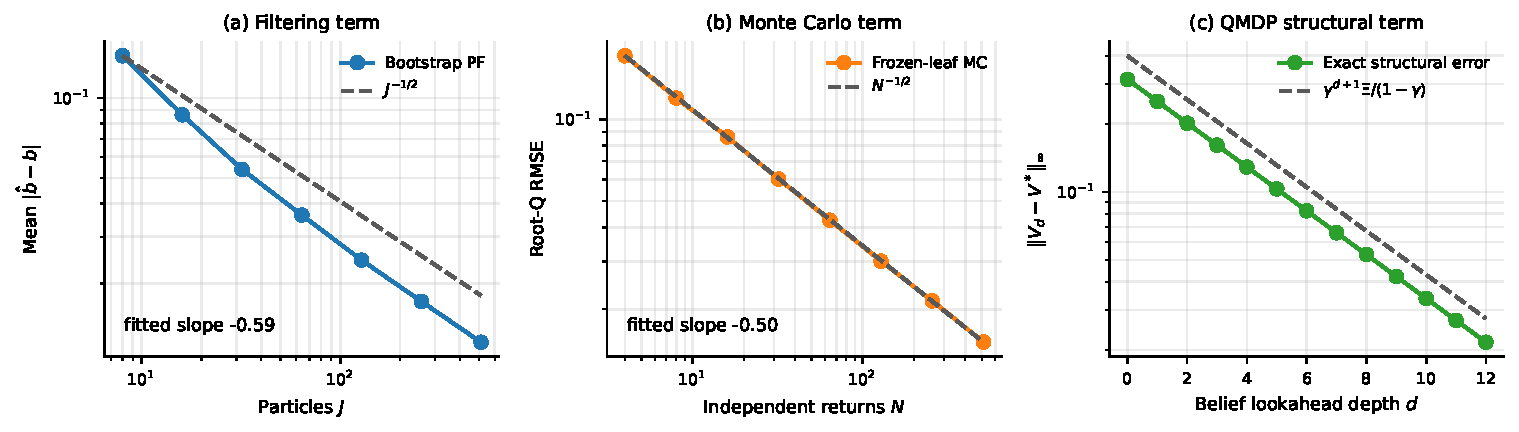
\includegraphics[width=\linewidth]{figures/ch08/Figures/theory_bound_audit.pdf}
    \caption[Empirical audit of regret decomposition error terms on Mixing Tiger]{\aigen{Empirical audit of the isolated filtering ($J$), Monte Carlo rollout ($N$), and structural planning-depth ($d$) error terms of Theorem~\ref{thm:final_regret_bound} on the Doeblin-mixing Tiger POMDP.}}
    \label{fig:theory_bound_audit}
\end{figure}

\begin{table}[t]
\centering
\caption[Empirical versus theoretical scaling rates on Mixing Tiger]{\aigen{Empirical versus theoretical scaling rates for the four terms of Theorem~\ref{thm:final_regret_bound} on the Doeblin-mixing Tiger POMDP.}}
\label{tab:fitted_rates}
\small
\begin{tabular}{lll}
\toprule
Decomposition Term & Empirical Scaling & Theoretical Rate \\
\midrule
Particle filtering ($J = 8 \to 512$) & $J^{-0.59}$ & $J^{-1/2}$ \\
Monte Carlo rollouts ($N = 4 \to 512$) & $N^{-0.50}$ & $N^{-1/2}$ \\
Structural depth bias ($d = 0 \to 12$) & $0.80^d$ per level & $\gamma^d = 0.80^d$ \\
Online MLE estimation ($\sum_{t=1}^T \varepsilon_{\mathrm{opt},t}$) & $T^{0.57}$ & $\widetilde O(\sqrt{T})$ \\
\bottomrule
\end{tabular}
\end{table}
\end{aigenblock}


\begin{table}[t]
\centering
\caption[Summary of Theorem~\ref{thm:final_regret_bound} assumptions across Chapter~\ref{ch:pomdp-control} environments]{Which experiments satisfy the assumptions of Theorem~\ref{thm:final_regret_bound}. \checkmark: holds; $\times$: fails; $\sim$: approximately.}
\label{tab:theory_coverage}
\small
\begin{tabular}{lccccl}
\toprule
Environment & Doeblin & $g_{\min}>0$ & Finite $\gA$ & Bounded $r$ & Role \\
\midrule
\aigen{Mixing Tiger} & \aigen{\checkmark} & \aigen{\checkmark} & \aigen{\checkmark} & \aigen{\checkmark} & \aigen{theory-valid audit} \\
HeartSteps & $\sim$ & $\sim$ & \checkmark & \checkmark & approximately valid \\
Double-integrator LQR & \checkmark & $\times$ & $\times$ & $\times$ & filtering diagnostic \\
MuJoCo & $\times$ & $\times$ & $\times$ & \checkmark & heuristic demonstration \\
\bottomrule
\end{tabular}
\end{table}

We instantiate \aigen{Algorithm~\ref{alg:pf_mcts}} using the \texttt{pypomp} \citep{pypomp2024github} package for particle-filtering primitives
with \aigen{weight-discounted particle filter (Algorithm~\ref{alg:dmop} in Chapter~\ref{ch:pomp-estimation}; \citealp{tan2024accelerated})} or VSMC \citep{naesseth18} gradient estimators. This allows us to employ highly optimized JAX implementations of the particle filter on GPU. We learn a neural dynamics
model online, maintain a particle approximation to the latent state posterior,
and use an actor and a critic trained with recurrent SAC-style updates \citep{ni2021recurrentbaseline} in the same vein as \cite{han2026neuralodesdemodels}.  In the experiments we use belief-tree depth $d=0$: each particle is rolled out at the state level under a learned actor and bootstrapped with a learned critic, rather than planning over a tree of particle beliefs.
With continuous actions and observations a depth-$d$ tree requires binning at a cost of up to $(|\gA|M)^d$ nodes, so this is the main practical gap from the theory.
Rollout planning corresponds to the QMDP end of the depth axis, whereas deeper belief planning reduces the structural bias.
\aigen{Appendix~\ref{sec:app08-planner-comparison} evaluates the analyzed belief-tree planner at depths $d > 0$ on finite active-sensing POMDPs against POMCP and Sparse-PFT. The practical deep RL instantiation is presented in Algorithm~\ref{alg:pf_mcts_practical}. All deep RL experiments were run on two RTX 3090 GPUs.}

\todoresolve{CAMERA-READY ITEM E3/E4: CONFIRM THAT THE PRACTICAL DEEP RL INSTANTIATION AND THE HYPERPARAMETER TABLES DISTINGUISH STATE-LEVEL ROLLOUT HORIZON L FROM BELIEF-TREE DEPTH d=0, AND VERIFY PLANNER COMPARISON CODE AGAINST REVISED DP-BACKUP PSEUDOCODE.}



\textbf{Double-integrator LQR.} We first study a partially observed double-integrator LQR.  The state contains
position and velocity, but the observation reveals only position. The
latent velocity is therefore not identifiable from the current observation alone. Different
velocities induce the same observation and can only be distinguished using
history.  This environment isolates the filtering problem.  The posterior
diagnostics in Figure \ref{fig:lqr-posterior-small} show that particle beliefs can track the latent state without access to memory, while failures occur when the system is unstable.
The GRU backbone improves this behavior relative to a memoryless MLP, suggesting that particle filtering and recurrent state representations are
complementary. More details and figures can be found in Appendix \ref{app:lqr}.

\textbf{HeartSteps.} We next evaluate the HeartSteps benchmark of \cite{gao2025activemeasuringreinforcementlearning} as an actively observable MDP with a latent reward
state, where the learner can choose to measure the state at a cost. \aigen{Algorithm~\ref{alg:pf_mcts}} is run in the never-measure regime. It never directly measures
the latent reward and must infer it from passive observations.  The strongest
benchmark is RLSVI-SMC/never-measure, which is specifically tailored to the
linear-Gaussian HeartSteps structure and uses hand-specified linear features.
Consequently, RLSVI-SMC performs best in most scenarios.  \aigen{Algorithm~\ref{alg:pf_mcts}} typically
improves over the baseline rollout but trails RLSVI-SMC because it must learn a deep
model, actor, and critic from data.  Dyna-ATMQ is not directly comparable as a
no-measure method. It actively measures the latent reward roughly half the time,
which gives it an informational advantage, but this advantage can be offset when
measurement has delayed negative effects on future engagement. More details and figures can be found in Appendix \ref{app:heartsteps}.


\begin{figure}[t]
    \centering
    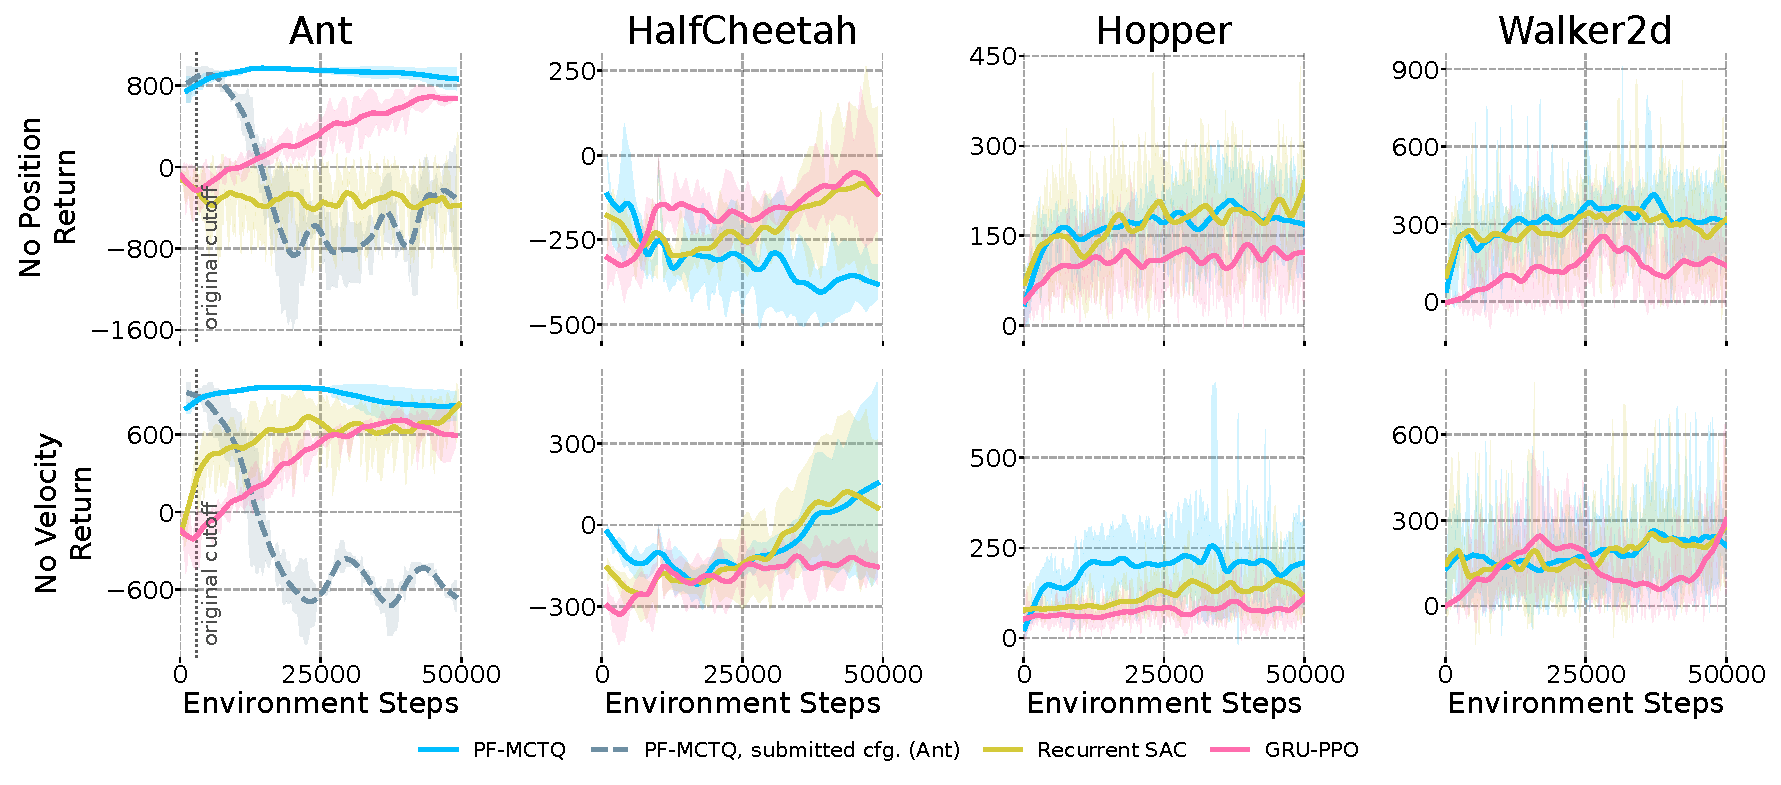
\includegraphics[width=\linewidth]{figures/ch08/Figures/mujoco_camera_ready.pdf}
    \caption[Partial-observation MuJoCo learning curves in the low-sample regime]{\aigen{Partial-observation MuJoCo learning curves in the low-sample regime across Ant, HalfCheetah, Hopper, and Walker2d with either position or velocity hidden. Non-Ant panels and baselines show smoothed per-episode returns across $5$ seeds ($\text{mean} \pm 1.96\,\mathrm{SD}/\sqrt{n}$). The Ant panels plot the $10$-episode rolling training return over the full $49.2\text{k}$-step horizon for the stabilized update-to-data configuration (solid, $3$ seeds) alongside the initial high-UTD configuration (dashed, $2$ complete seeds, which peaks near $3\text{k}$ steps indicated by the vertical dotted line before collapsing).}}
    \label{fig:mujoco}
\end{figure}

\textbf{MuJoCo partial-observation control.}
Finally, we evaluate Ant, HalfCheetah, Hopper, and Walker2d with either position
or velocity components removed from the observation.  We compare \aigen{Algorithm~\ref{alg:pf_mcts}} to
Recurrent SAC and GRU-PPO baselines from the recurrent model-free POMDP
benchmarking literature~\citep{ni2021recurrentbaseline}.  These are strong comparators:
they are designed to solve POMDPs by learning a recurrent history representation
directly from reward. Figure~\ref{fig:mujoco} shows that \aigen{Algorithm~\ref{alg:pf_mcts}} is competitive in
the ultra-low-sample regime.  \aigen{On Ant, the initial high-update-frequency configuration reaches a high $10$-episode rolling return near $3\text{k}$ steps ($908$ with position hidden and $897$ with velocity hidden) but subsequently destabilizes and collapses under continued training ($-448$ and $-648$ at $49.2\text{k}$ steps). Regularizing the update schedule (reducing the policy update-to-data ratio to $1/10$ with online model updates and weight decay, detailed in Appendix~\ref{sec:app08-ant-full}) preserves rapid early learning ($825$ and $882$ at $3\text{k}$ steps, rising to $960$ and $962$ at $20\text{k}$ steps) while maintaining stable returns through the end of the $49.2\text{k}$-step horizon ($868$ and $816$ rolling return at $49.2\text{k}$ steps, with final $10$-episode evaluation returns of $862$ and $767$).}
\todoresolve{CAMERA-READY ITEM E4: VERIFY THE EXACT CONFIG DIFFERENCE BETWEEN THE INITIAL AND STABILIZED ANT CONFIGS (UTD 1/10 PLUS ONLINE MODEL UPDATES AND WEIGHT DECAY) IN THE CONTROL REPO LOGS.}
On Hopper and
Walker2d, \aigen{Algorithm~\ref{alg:pf_mcts}} is broadly competitive with Recurrent SAC and usually stronger
than GRU-PPO early in training.  HalfCheetah is more mixed: \aigen{Algorithm~\ref{alg:pf_mcts}} performs well
when velocity is hidden but struggles when position is hidden, suggesting that
model bias and rollout error can dominate when the omitted coordinates are
crucial for short-horizon prediction.


\begin{aigenblock}
Table~\ref{tab:ch08_runtime} reports the measured wall-clock training cost on a single RTX 3090 GPU for the position-hidden Ant benchmark. The stabilized instantiation of Algorithm~\ref{alg:pf_mcts_practical} incurs approximately $13\%$ higher per-step training time than Recurrent SAC ($58.7\text{ s}$ versus $52.0\text{ s}$ per $1000$ environment steps) in addition to a $132.1\text{ s}$ warm-start initialization, whereas on-policy GRU-PPO runs substantially faster per step ($4.4\text{ s}$ per $1000$ steps) at the cost of much lower sample efficiency.

\begin{table}[t]
\centering
\caption[Wall-clock training runtime on partial-observation MuJoCo Ant]{\aigen{Measured wall-clock runtime on a single RTX 3090 GPU (MuJoCo Ant, position hidden, matched end-to-end collection and gradient updates).}}
\label{tab:ch08_runtime}
\small
\begin{tabular}{lrrr}
\toprule
Method & Warm-Start Init (s) & Train Time (s / 1k steps) & Throughput (steps / s) \\
\midrule
Algorithm~\ref{alg:pf_mcts_practical} (stabilized config) & 132.1 & 58.7 & 17.0 \\
Algorithm~\ref{alg:pf_mcts_practical} (initial config) & 139.6 & 50.2 & 19.9 \\
Recurrent SAC & 12.1 & 52.0 & 19.2 \\
GRU-PPO & 2.6 & 4.4 & 228.5 \\
\bottomrule
\end{tabular}
\end{table}
\end{aigenblock}

Overall, these results show that particle filtering and model-based planning can be implemented on top of existing deep RL algorithms and can yield sample-efficiency gains in partially observed control.  The results should not be read as a claim
of asymptotic dominance over recurrent model-free RL.  Rather, they show that the
theoretical learning--filtering--planning pipeline can be made operational in
standard deep RL benchmarks.



\section{Discussion}
\label{sec:conclusion}

We presented an online model-based POMDP pipeline that combines particle filtering, latent-dynamics learning, and approximate planning with an end-to-end regret bound. We decompose regret into model estimation error, particle approximation error, Monte Carlo planning error, and QMDP structural bias, clarifying how statistical and computational budgets affect performance. The resulting framework provides a practical bridge between POMDP theory and modern model-based deep RL. Experiments with a simplified rollout-based implementation show that this theoretically motivated pipeline can be made operational and competitive in low-sample partially observed control.

\textbf{Limitations.} Our analysis relies on the Doeblin mixing condition and bounded observation densities, which ensure passive state coverage and obviate the need for strategic exploration.
These assumptions fail in many POMDPs.
In item search with exact observations the observation density is not bounded below, and a particle set of size $J$ misses the true location among $K$ with probability $(1-1/K)^J$, while in Light--Dark-type problems, where information must be actively gathered, $\Xi_\theta$ is large and shallow planning never gathers it \aigen{(see the controlled stress tests in Appendix~\ref{sec:app08-stress-tests})}.
Second, the bounded reward assumption excludes settings such as LQG.
Third, the deep RL experiments run at depth $d=0$ with a learned critic and actor, so they sit at the QMDP end of the analyzed algorithm, and our guarantees cover non-adaptive (e.g., uniform) rather than UCT-style action selection inside the tree.
\aigen{In Appendix~\ref{sec:app08-planner-comparison}, we confirm empirically on multi-step active-sensing POMDPs that UCB1 action selection within the belief tree outperforms uniform exploration at a matched simulation budget, demonstrating that uniform exploration is purely a theoretical proof device.}
Natural extensions are strategic exploration to relax the assumptions on the dynamics, unbounded rewards, and guarantees for adaptive tree search.